%% The first command in your LaTeX source must be the \documentclass command.
\documentclass[sigconf,authorversion]{acmart}
%% NOTE that a single column version may be required for
%% submission and peer review. This can be done by changing
%% the \doucmentclass[...]{acmart} in this template to
%% \documentclass[manuscript,screen,review]{acmart}

\begin{document}
\settopmatter{printacmref=false}
\setcopyright{none}
\renewcommand\footnotetextcopyrightpermission[1]{}
\pagestyle{plain}
\title{Progress Report for CSS 586 Course Project: \\
Modeling Latent Patterns in Music}

%%
%% The "author" command and its associated commands are used to define
%% the authors and their affiliations.
%% Of note is the shared affiliation of the first two authors, and the
%% "authornote" and "authornotemark" commands
%% used to denote shared contribution to the research.

\author{Alex Kyllo}
\email{akyllo@uw.edu}
\affiliation{%
  \institution{University of Washington}
  \city{Bothell}
  \state{WA}
  \country{USA}
}

\begin{abstract}
This report explores recent research in modeling music with deep learning and
provides a progress report on a course project to train a generative model of
classical and popular music on the MusicNet and Lakh MIDI datasets.
\end{abstract}

\keywords{deep learning, sequence learning, generative modeling, recurrent neural networks, music, MIDI}

\maketitle

\section{Introduction}

Machine learning models of music have interesting applications in music
information retrieval and creative tools for musical artists and educators.
Music is complex and challenging to model because it exhibits a hierarchy of
recurring patterns.

Depending on the task, machine learning models of music may be trained on the
audio signal itself, either in a time domain or a frequency domain
representation, or they may be trained on a digital symbolic representation of
music, the most common of which is MIDI (Musical Instrument Digital Interface)
notation. MIDI is an encoding of music as streams of bytes in one or more tracks
or channels, each representing a sequence of 128 possible pitch values, along
with timing, pressure and instrument values. A music transcription model may
convert an audio signal into MIDI, which can easily be converted into other
symbolic representations such as sheet music for human performers to read from,
while a synthesizer model can convert MIDI representations into audio signals.

\section{Related Work}

Google's \href{https://magenta.tensorflow.org/}{Magenta} is an umbrella project
for music deep learning research and development of software tools to expose
these models for use by creative artists and students.

MusicVAE is a variational LSTM autoencoder for MIDI that incorporates a
novel hierarchical structure using a ``composer'' recurrent layer in its encoder
model to better capture structure at multiple
levels \cite{roberts_hierarchical_2018}.

MuseGAN \cite{dong2017musegan} is an application of Generative Adversarial
Networks to polyphonic MIDI music generation, trained on four-bar phrases of a
multi-track pianoroll representation of rock songs from the Lakh Midi Dataset
\cite{raffel_learning-based_2016}.

Music Transformer is a generative model that borrows its approach from the
Natural Language Processing (NLP) domain, using an attention network to model
MIDI music as a sequence of discrete tokens with relative positional dependencies
\cite{huang_music_2018}.

A major advantage of working with the symbolic representation of music is that
it is of far lower dimensionality than the raw audio waveforms of a recorded
performance, which makes it less computationally expensive. However, there are
many aspects of musical performance that are not captured by a symbolic
representation, so the expressiveness of symbolic generative models is
constrained \cite{manzelli_conditioning_2018}.

Other research has focused on modeling raw audio waveforms directly. WaveNet is
a causal convolutional neural network for generating raw audio waveforms,
developed by Google DeepMind, which achieves state of the art performance in
generating natural sounding speech from text, but is also capable of generating
short, realistic snippets of audio music \cite{oord_wavenet_2016}.

Another model named SampleRNN generates raw audio waveforms using a three-tier
hierarchy of gated recurrent units (GRU) to model recurrent structure at
multiple temporal resolutions \cite{mehri_samplernn_2017}.

Jukebox by OpenAI utilizes a vector-quantized variational autoencoder (VQ-VAE)
to compress raw audio into a sequence of discrete codes and models these
sequences using autoregressive transformers to generate music
\cite{dhariwal2020jukebox}.

Audio data can also be modeled in the frequency domain through the use of
Fourier analysis. The recent MelNet model is trained on spectrograms and can
learn musical structures such as melody and harmony and variations in volume,
timbre and rhythm \cite{vasquez2019melnet}.

Prior work points out that the division between symbolic music notes and the
sounds of music is analogous to the division between symbolic language and
utterances in speech, which may inspire ideas for combining the two approaches
\cite{hawthorne2019enabling}. A paper from Boston University describes an effort
to combine the symbolic and waveform approaches to music modeling, by training
an LSTM to learn melodic structure of different styles of music, then providing
generations from this model as conditioning inputs to a WaveNet-based raw audio
generator \cite{manzelli_conditioning_2018}.

\section{Planned Methods}

\subsection{Datasets}

\subsection{Data Preprocessing}

This project will focus on the generative modeling of symbolic music using MIDI
data, because of the advantages of symbolic music models in representing
long-term structure in musical compositions to produce generations with coherent
use of repetition over long time scales.

Several choices must be made in how to preprocess MIDI files into training
examples for a neural network. In order to accommodate polyphonic music, we will
convert each MIDI file into a pianoroll representation, wherein each instrument
track is a sparse matrix of the velocity values for each of 128 possible pitch
levels at each timestep. Because songs are typically at least a few minutes long
and of widely varying length, we will crop songs into equal-length phrases.

The result of this preprocessing is that each training example will be a 3D
tensor of shape (tracks x notes x ticks) and stacking the training examples will
produce a 4D tensor, which is also typically the dimension of image data
tensors in machine learning.

\begin{figure}[h]
  \centering
  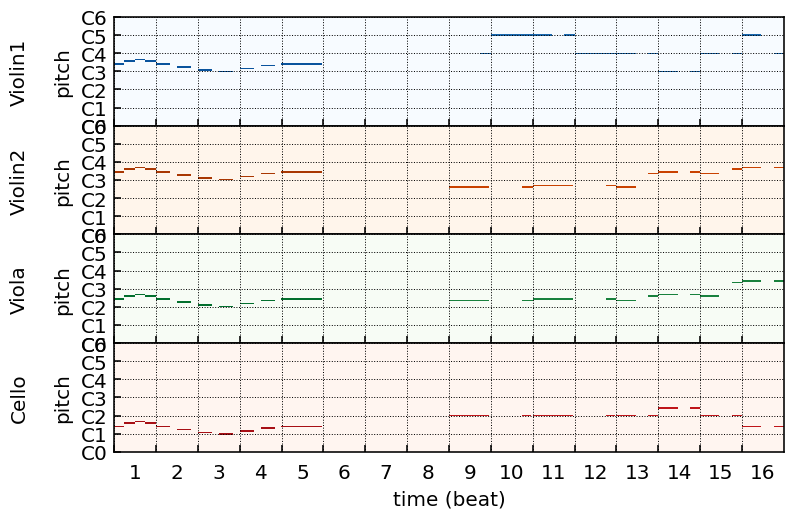
\includegraphics[width=\linewidth]{first_four_bars.png}
  \caption{The first four bars of Beethoven's Serioso String Quartet}
  \Description{A pianoroll representation of cello, viola and violin parts.}
\end{figure}

Data augmentation is also possible--the literature suggests augmentation via
pitch shifting the entire training example up or down by up to six semitones,
and increasing or reducing the speed by up to 10\% in order to create additional
training examples and reduce overfitting \cite{oore_this_2018}.

\subsection{Model Fitting}

We will explore several modeling approaches to generating symbolic music:

\begin{itemize}
  \item{Sliding window sequence prediction with RNNs (LSTM/GRU)}
  \item{Sliding window sequence prediction with Transformers}
  \item{Latent space interpolation with Sequential VAEs}
  \item{Latent space interpolation with Sequential GANs}
\end{itemize}

\subsection{Model Evaluation}

Evaluation of generative models is challenging because there is no equivalent of
an accuracy metric like what is used in supervised learning. Generative models
are typically evaluated using a combination of qualitative metrics whereby human
judges rate the quality of the generated examples (essentially a Turing test),
and quantitative metrics that assess the differences in the parametric
distributions of generated and real examples. Yang and Lerch (2020) proposes a
set of metrics informed by music theory, for probabilistically evaluating how
similar the generations are to known sample distributions of real music
\cite{yang_evaluation_2020}. These metrics include counts, ranges, histograms
and transition matrices of pitches and note lengths, then the Kullback-Leibler
divergence and overlapping area of the probability density functions are use to
compare against known reference distributions per musical genre
\cite{yang_evaluation_2020}. Due to the cost and time requirements associated
with designing a human subjects experiment, we plan to utilize this quantitative
approach to generation quality assessment.

\section{Progress and Remaining Work}

\bibliographystyle{ACM-Reference-Format}
\bibliography{progress-alex}

\end{document}
\endinput
